\documentclass[tikz,border=4pt]{standalone}
\usepackage{amsmath,amssymb}
\usetikzlibrary{arrows.meta}
\begin{document}
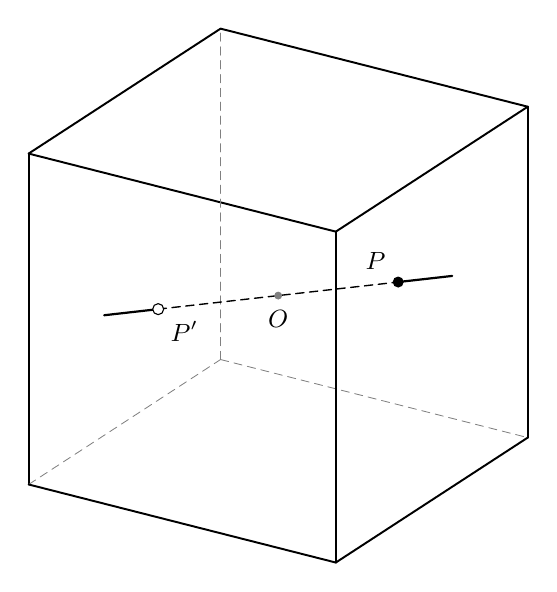
\begin{tikzpicture}[line cap=round,line join=round]
\draw[line width=0.7pt] (-3.1693,-2.3988) -- (-3.1693,1.8035);
\draw[densely dashed,gray,line width=0.3pt] (-3.1693,-2.3988) -- (-0.7317,-0.8121);
\draw[line width=0.7pt] (-3.1693,-2.3988) -- (0.7317,-3.3902);
\draw[line width=0.7pt] (-3.1693,1.8035) -- (-0.7317,3.3902);
\draw[line width=0.7pt] (-3.1693,1.8035) -- (0.7317,0.8121);
\draw[densely dashed,gray,line width=0.3pt] (-0.7317,-0.8121) -- (-0.7317,3.3902);
\draw[densely dashed,gray,line width=0.3pt] (-0.7317,-0.8121) -- (3.1693,-1.8035);
\draw[line width=0.7pt] (-0.7317,3.3902) -- (3.1693,2.3988);
\draw[line width=0.7pt] (0.7317,-3.3902) -- (0.7317,0.8121);
\draw[line width=0.7pt] (0.7317,-3.3902) -- (3.1693,-1.8035);
\draw[line width=0.7pt] (0.7317,0.8121) -- (3.1693,2.3988);
\draw[line width=0.7pt] (3.1693,-1.8035) -- (3.1693,2.3988);
\draw[line width=0.5pt,densely dashed] (-1.5239,-0.1721) -- (1.5239,0.1721);
\draw[line width=0.8pt] (1.5239,0.1721) -- (2.2097,0.2496);
\draw[line width=0.8pt] (-1.5239,-0.1721) -- (-2.2097,-0.2496);
\fill (1.5239,0.1721) circle (0.07) node[above left=1pt,font=\small] {$P$};
\draw[fill=white,line width=0.4pt] (-1.5239,-0.1721) circle (0.07) node[below right=1pt,font=\small] {$P'$};
\fill[gray] (0.0000,0.0000) circle (0.05) node[below=2pt,font=\small,black] {$O$};
\end{tikzpicture}
\end{document}
